\chapter{Shapes}

Once you know how to show a dot on the screen, other shapes are easy. (If you don't, review chapter \ref{chapter:positions}.) Most mathematical shapes can be drawn on the screen. The classes to do that are in the green folder Esenthel Engine $\Rightarrow$ Math $\Rightarrow$ Shapes.

Not all available shapes are intended for display in 2D. Some classes, like \eeClass{Ball} and \eeClass{Tube}, are intended for 3D development. For now, we will focus on 2D shapes like \eeClass{Circle}, \eeClass{Edge} (line), \eeClass{Quad}, \eeClass{Rectangle} and \eeClass{Triangle}.

\section{Circle}
To draw a circle you need a radius(r) and a position(pos). The radius is a \eeClass{float}, the position a \eeClass{Vec2}. There is more than one way to pass these to a circle:

\begin{code}
// using the constructor, with r(float), pos.x(float), pos.y(float)
Circle c(0.1, 0, 0);

// using the constructor, with r(float), pos(Vec2)
Circle c(0.1, Vec2(0, 0));

// during the coarse of the application
c.set(0.1, 0, 0);
c.set(0.1, Vec2(0, 0));

// directly changing the variables
c.r = 0.1;
c.pos = Vec2(0, 0);
\end{code}

\subsection{Methods}
The set function aside, there are also methods available to retrieve the current area or perimeter, and to draw the circle on the screen.

\begin{code}
// retrieve area and perimeter
float a = c.area();
float b = c.perimeter();

// draw a blue circle on the screen
c.draw(BLUE);

// draw the perimeter only
c.draw(BLUE, false);
\end{code}

There's something remarkable about the \eeFunc{draw} method! It can be used with one as well as with two methods. To see how this is possible, look at the declaration of this method, which can be found at Esenthel Engine $\Rightarrow$ Math $\Rightarrow$ Shapes $\Rightarrow$ Circle:

\begin{code}
void draw(C Color & color, Bool fill = true, Int resolution = -1) C;
\end{code}

The first argument is a \eeClass{Color}. The second argument is a \eeClass{bool} named `fill'. You might suspect this means whether or not you desire to draw the circle as a perimeter or an area. And of course you're right. Only, the argument doesn't stop there: it has a value assigned ( = true). This is called a default value. If you agree with the default, you don't gave to explicitly pass true as an argument. Only when you don't agree, you will have to pass false.

\begin{note}
The third argument (resolution) is also optional. Experiment with several values to find out what is does. (Try values like 2, 3, 8, 14, \ldots)
\end{note}

\subsection{Math}
You can do math with circles. There are operators like \eeOpp{+=}, \eeOpp{-=}, \eeOpp{/=} and \eeOpp{*=}, which can be used to alter the radius or the position. How do you know which value will be altered? Well, if you add a float to a circle, the radius change. When you add a \eeClass{Vec2} this will later the position.

\begin{code}
Vec2 pos(0.1, 0);
Circle c(0.1, pos);

// move the circle 0.1 units to the right
c += pos;
// move the circle 0.2 units down
c -= Vec2(0, 0.2);
// double the radius
c *= 2;
\end{code}

\subsection{Exercises}
Recreate the following image by drawing circles on the screen. If you like a challenge, try creating a more fitting mouth with the method \eeFunc{drawPie}.

\begin{figure}[h]
\centering
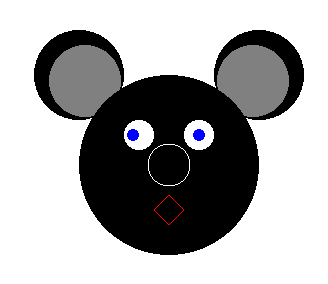
\includegraphics[width=0.4\linewidth]{images/circle_exercise.png}
\caption[]{Pay attention to the eyes!}
\label{fig:pos2D}
\end{figure}

\section{Edge2}
An \eeClass{Edge2} is a line. Just as with \eeClass{Vec2}, the '2' is important. The code will still be valid when you use an \eeClass{Edge} instead of an \eeClass{Edge2}, but that class is intended for drawing in 3D instead. To define an \eeClass{Edge2}, you need two points (\eeClass{Vec2}), being the beginning and the end. Esenthel offers two methods to pass these to the object:

\begin{code}
Edge2 e1;
Edge2 e2;

// using newly created vectors ...
e1.set(Vec2(0, 0), Vec2(0.1, 0.1));

// ... or existing vectors
Vec2 pos1(0.3, 0.6);
Vec2 pos2(0.1, 0.2);
e1.set(pos1, pos2);

// set all x and y values as floats
e2.set(-0.4, 0.2, -0.7, 0.9;
\end{code}

\subsection{Methods}
An \eeClass{Edge2} provides several neat methods. The most obvious will be \eeFunc{draw()}:

\begin{code}
line1.draw(PURPLE    ); // draw a purple line
line2.draw(GREEN, 0.1); // draw a green line, with width 0.1
line3.draw(GREEN, RED); // draw a line that starts out green but fades to read
\end{code}

Other methods of interest are \eeFunc{center()}, \eeFunc{delta()}, \eeFunc{dir()} and \eeFunc{length()}. All of them can be found in $\Rightarrow$ Math $\Rightarrow$ Shapes $\Rightarrow$ Edge.

\subsection{Exercises}

The methods \eeFunc{Sin()} en \eeFunc{Cos()} allow you to retrieve the sine and cosine from any value. This is most fun when that value is the current time. The result over time is a value which moves smoothly between -1 and 1.

\begin{code}
float x = Sin(Time.curTime());
float y = Cos(Time.curTime());
\end{code}

\begin{enumerate}
\item The code above illustrates how to use the sine and cosine with the current time. Create an application which shows a line, starting from the middle of the screen towards the current value of sine and cosine for the x and y value of the ending.
\item Change the width of the line.
\item Make the line move at double speed.
\item Decrease the length of the line. 
\item \textit{(This will be a bit harder)} Try to create an analog watch.
\end{enumerate}

Take a look at Esenthel Engine $\Rightarrow$ Math $\Rightarrow$ Shapes $\Rightarrow$ Edge. Examine the method \eeFunc{lerp(float s)}. This function needs an argument between zero and one, and return a position on the line.

\begin{enumerate}
\item Define an \eeClass{Edge2} and a \eeClass{float} with value zero.
\item In the init function, assign a start and end position to your line.
\item In the update function you increase the float with \eeClass{Time.d()}. When the float value is larger than 1, is should be assigned 0.
\item Draw the line in black with a width of 0.05. Construct a \eeClass{Vec2} with the result of \eeFunc{lerp()}. The argument of the method should be your float. Draw this point in red, also with a width of 0.05.
\end{enumerate}

Draw a triangle on the screen.

\section{Rect}
The last shape in the chapter is a rectangle: \eeClass{Rect}. You will end up using this shape quite a lot, because a rectangle happens to be the shape of most gui elements, like buttons, windows and images.

After the last exercise, you know that you need 3 positions to draw a triangle. Logic dictates a rectangle requires 4 positions, right? But there's one property of a rectangle that makes it a lot easier: all corners have an angle of 90\%. This means that when you pass the lower left corner and the upper right corner, there is enough information to find the two remaining corner positions.

\begin{figure}[h]
\centering
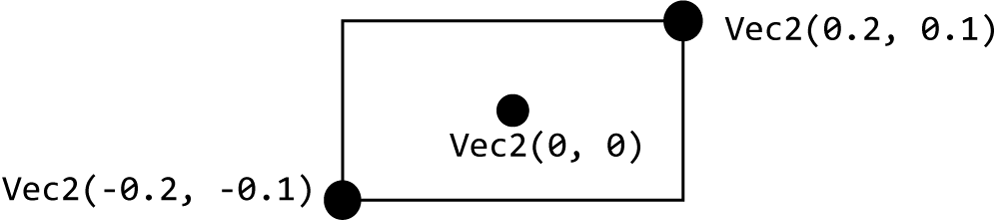
\includegraphics[width=0.8\linewidth]{images/rectangle.png}
\caption[]{The corners of a rectangle}
\label{fig:rect}
\end{figure}

This means a rectangle can be created like this:

\begin{code}
Rect(Vec2(-0.2, -0.1), Vec2(0.2, 0.1)).draw(BLACK, false);
\end{code}

Again there is a draw function with the color as the first argument. And optionally you can draw only the perimeter of the rectangle. Just as with \eeClass{Edge2} there is another version of the constructor allowing you to enter the x- and y-coordinates one by one.

\begin{code}
Rect(-0.2, -0.1, 0.2, 0.1).draw(BLACK);
\end{code}

\subsection{A moving Rectangle}
If you want to draw an image on the screen, it will require a rectangle. As such, a rectangle will be the basis of almost every element on your screen. It will often come in handy to have a special class for movable rectangles. As an example, we'll create a rectangle which can be moved with the arrow keys.

Rectangles have one big disadvantage when you try to move them. Instead of a central position, both corners have to be moved. This is why we often use a \eeClass{Vec2} to remember the center position. As an extra, this class will remember its color.


\begin{code}
class movableRect {
  	Vec2 pos;
	Color color;
}
\end{code}

This class can be extended with a create, update and draw methods. The create method can be used to pass the color and the starting position to the object. This starting position already has a default value, so you can use the create method without it.

\begin{code}
void create(C Color & color, C Vec2 & pos = 0) {
  	T.color = color;
	T.pos = pos;
}
\end{code}

\begin{note}
There some other new stuff in this method. The \& sign indicates that the color and pos will be passed as a reference. The character \eeFunc{C} means we will not change the value that was passed into the method. You will learn more about this in one of the next chapters. Within the function, the character \eeFunc{T} is used to solve a practical problem. The class and the method both have a variable named `color'. This makes it impossible for the compiler to know what variable you mean. You could rename one of them, but that makes the code harder to read. A more elegant solution is to add \eeFunc{T.} before the class variable. T stands for `this' and by that we mean `this class'. The version without \eeFunc{T.} will be the local variable, passed into the method.
\end{note}

Within the update method, the position can be changed by using the arrow-keys. You came across this code before, in chapter \ref{chapter:keyboardInteractie}.

\begin{code}
void update() {
	if(Kb.b(KB_LEFT )) pos.x -= Time.d();
	if(Kb.b(KB_RIGHT)) pos.x += Time.d();
	if(Kb.b(KB_UP   )) pos.y += Time.d();
	if(Kb.b(KB_DOWN )) pos.y -= Time.d();
}
\end{code}

The final thing we need is a draw function. Notice that this is the only place we actually create a rectangle. That's because we don't really need the whole rectangle in the other methods. This could be different if, for example, we need to check if the rectangle hits another object. So you could add a real \eeClass{Rect} to this class, but right now it is not needed.

\begin{code}
void draw() {
  Rect(pos - Vec2(0.2, 0.1), pos + Vec2(0.2, 0.1)).draw(color);
}
\end{code}

As you see, we use the position `pos' when we create the rectangle. The position will be the middle of the rectangle. But we still need to define the corner. This can be done be subtracting and adding the same value from the position. In this case the value is literal, but a more advanced class could just define a \eeClass{Vec2 size} and use that instead. That would make it easy to define movable rectangles of different sizes.

The whole class is listed again below. It is the first time in this course we actually create a new class, so be sure you understand what is going on. And pay attention to the keywords \eeClass{private} and \eeClass{public}. You should know those from an introductory c++ course. We will talk more about those later on, but remember they are part of a good programming style.

\begin{code}
class movableRect {
private:
  Vec2 pos, size;
	Color color;
	
public:
  void create(C Color & color, C Vec2 & pos = 0, C Vec2 & size = Vec2(0.1, 0.1)) {
	  T.color = color;
		T.pos   = pos  ;
		T.size  = size ;
	}
	
	void update() {
		if(Kb.b(KB_LEFT )) pos.x -= Time.d();
		if(Kb.b(KB_RIGHT)) pos.x += Time.d();
		if(Kb.b(KB_UP   )) pos.y += Time.d();
		if(Kb.b(KB_DOWN )) pos.y -= Time.d();
	}
	
	void draw() {
		Rect(pos - size, pos + size).draw(color);
	}
}
\end{code}
	
\subsection{Exercises}

\begin{enumerate}
\item Recreate this screen in an application:

\begin{figure}[h]
\centering
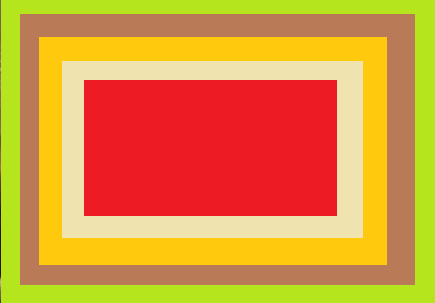
\includegraphics[width=0.4\linewidth]{images/nested_rectangles.png}
\caption[]{Rectangles}
\label{fig:nested_rect}
\end{figure}

\item Add a pink square to the application, using the newly created class \eeClass{movableRect}.
\item \textit{(A bit harder)} Be sure the square cannot move outside of the screen.
\end{enumerate}

\section{Cuts}

A function that is used very often in combination with shapes is \eeFunc{Cuts}. There are quite a lot of different versions of this function, but its meaning is always the same: do two shapes overlap, or don't they? The \eeFunc{Cuts} function allows you to check if a dot is inside a circle, if a circle (partially) overlaps a rectangle, if a line cuts a rectangle and so on. 

To check if a dot is inside a circle, use the code below:

\begin{code}
Vec2 pos(0.1, 0.1);
Circle area(0.3, Vec2(0));

if(Cuts(pos, area)) area.draw(RED);
\end{code}

Of course, in this example it is already certain the dot will always be inside the circle. But you could use the same principle to see if the mouse pointer is inside the circle, like this:

\begin{code}
Circle area(0.1, Vec2(0));

if(Cuts(Ms.pos(), area)) area.draw(RED);
else area.draw(BLACK);
\end{code}

The code above is the starting point for many possible interactions. Often, this will be in combination with other rules. Try to find out what the code below does:

\begin{code}
Rect button(Vec2(-0.2, -0.1), Vec2(0.2, 0.1));
bool hover = false;

// in the update function:
if (Cuts(Ms.pos(), button)) {
    hover = true;
	if(Ms.bp(0)) exit();
} else hover = false;

// in the draw function:
if(hover) {
  button.draw(Color(0, 255, 0));
} else {
  button.draw(Color(0, 155, 0));
}
\end{code}

\begin{exercise}
\begin{enumerate}
\item Create an application with 3 circles, each one below the other. Only the border of the circles is drawn, unless the mouse pointer is in that particular circle. In which case you draw a filled circle.
\item Make the circles move slowly to the right as long as the mouse pointer is inside the circle.
\item Create an integer `score'. When the circle goes over the right side of the screen, increase the score by one and place the circle back in the middle.
\end{enumerate}

\textit{(A bit harder) } Create your own class that behaves like a button, with a hover effect. The button also needs a line of text, which will be set by the create function.
\end{exercise}



